
\section{\boldmath Selection}

\subsection{Dataset}
In this analysis, 
the dataset with an integrated luminosity of $3.0~\rm fb^{-1}$ collected by the \lhcb experiment~\cite{Alves:2008zz,LHCb-DP-2014-002} in 2011 and 2012 is used. 
The processes of \LbLckkpi and \LbLcDs are reconstructed  with software versions of \texttt{Reco14} Stripping21(r1) and \davinci v42r6p1 for 2012(2011) data. 
In the reconstruction, 
the momentum scale calibration is used. 
In both data and MC, 
we use a decay tree fitter to constrain the $\Lb$ to originate from the primary vertex, 
and the invariant mass  to the known value for each open charm candidate~\cite{PDG}. 
For the study of the relevant resonance structures, 
further constraint of the mass of $\Lb$ to the PDG value is also applied. 
The resulting four momenta of final states are used to compute the invariant masses of the intermediate resonances in \LbLckkpi decays. 

For the Monte Carlo (MC) study, 
2.2  million events for \LbLckkpi 
and 0.7 million for \LbLcDs(\Dskkpi) are generated in the simulated $pp$ collisions at $\sqrt{s}=7\tev$ and 8\tev. 
Besides, 
the \LbLckkpi channel is also generated via intermediate states: 
1.4 million with $K(892)^{*0}\to K^+\pi^-$ resonance and 1.4 million with also $a_1(1260)^+\to K(892)^{*0}K^-$ resonance. 

The fragmentation and hadronization are simulated by \pythia 8, 
the decay by \evtgen and the detector response by \geant. 
For the reconstruction, 
the same software versions are adopted as used for data.

\subsection{Preselection}
\begin{table}[b]
\centering
\caption{Trigger lines for the \LbLckkpi and \LbLcDs candidates.}
\vspace{0.2cm}
\begin{tabular}{ll}\hline\hline
L0&$\Lb$ L0HadronDecision(TOS) \\
Hlt1&$\Lb$ TrackAllL0Decision(TOS)\\
Hlt2&$\Lb$ Topo2(3,4)BodyBBDTDecision(TOS)\\\hline
\end{tabular}
\label{tab:trigger}
\end{table}

The adopted trigger lines for \LbLckkpi and \LbLcDs are the same and listed in Table~\ref{tab:trigger}. 
The \lone trigger is chosen so that the systematic uncertainty of L0 efficiency could cancel a lot in the normalization ratio. 
And the 4-body topological line is also used considering the possible resonance state.
In those two decays, the \Lc is reconstructed as a combination of $\proton K^-  \pi^+$. 
Then \Lc is combined with $\Dsm$ or $\Kp \Km \pi^-$ for the reconstruction of \Lb.
Those decays through \LbLckkpi pass the \texttt{Lb2LcKKPiLc2PKPiBeauty2CharmLine} stripping line, 
while the \LbLcDs candidates pass the \texttt{Lb2LcDD2HHHPIDBeauty2CharmLine}. 


\begin{table}[!bth]
\centering
\caption{Stripping selections on the \LbLckkpi and \LbLcDs candidates.}
\vspace{0.2cm}
\begin{tabular}{lccc}
\hline\hline
\#& Selection variable& \LbLckkpi  &\LbLcDs   \\\hline
\multicolumn{4}{c}{all basic particles}\\\hline
1 &  $\chi^2_{trk}$/ndof &  \multicolumn{2}{c}{$<3$}  \\
2 & $P$(ghost) &  \multicolumn{2}{c}{$<0.4$}   \\
3 & \pt &  \multicolumn{2}{c}{$> 100$\mevc} \\
4 & $p$ &  \multicolumn{2}{c}{$>1000$\mevc}   \\
5 &   $\chi^2_{IP}$ &   \multicolumn{2}{c}{$> 4$}     \\\hline
\multicolumn{4}{c}{\Lc selection}\\\hline
6& \pt($K$)+\pt($p$)+\pt($\pi$)&  \multicolumn{2}{c}{$> 1800$\mevc}  \\
7& $\chi^2_{vtx}$/ndof &   \multicolumn{2}{c}{$< 10$}  \\
8&$\chi^2_{FD}$  &\multicolumn{2}{c}{$> 36$}   \\
9& $|M_{rec}-M_{pdg}|$ &  \multicolumn{2}{c}{$< 100$ \mevcc }  \\
10& one track with &     \multicolumn{2}{c}{$\pt > 500$\mevc, $p > 5000$\mevc}  \\
11& $PIDp(\proton)$ & \multicolumn{2}{c}{$> -10$}  \\
12& $PIDK(K^-)$ & \multicolumn{2}{c}{$> -10$} \\
13& $PIDK(\pi^+)$ & \multicolumn{2}{c}{$< 20$} \\\hline
\multicolumn{4}{c}{\Kp, \Km, $\pi^-$ from \Lb or $\Ds$}\\\hline
14& $p$ & $> 2000$\mevc& $>1000$\mevc \\
15& $PIDK(\Kp,\Km)$ & $>-2$ & $>-10$\\
16& $PIDK(\pi^-)$ & $<10$ & $<20$ \\ \hline
\multicolumn{4}{c}{$\Kp\Km\pi^-$ vertex cut}\\ \hline
17& $\chi^2_{vtx}$/ndof &$<8$&$<10$\\
18 & $\chi^2_{FD}$ & $>16$ &$>36$\\
19 & $BPV cos(\theta_p)$& $>0.98$ &$>0$\\
20 & $BPV VDRHO$& $> 0.1$mm &---\\
21 & $BPV VDZ$& $> 2.0$mm &---\\
22 & $\pt$(daughtersum)& $>1250$\mevc&$>1800$\mevc\\
23 & invariant mass & $< 3000$\mevcc&($1769.62,2068.49$)\mevcc \\
24 & two track with& $\pt>300$\mevc &---\\
25 &  one track with &\multicolumn{2}{c}{$\pt > 500$\mevc, $p > 5000$\mevc}\\\hline
\multicolumn{4}{c}{\Lb selections}\\\hline
26&$\chi^2_{vtx}$/ndof & \multicolumn{2}{c}{ $< 10$}\\
27&$\tau$ & \multicolumn{2}{c}{$> 0.2$ ps}\\
28&$\chi^2_{IP}$& \multicolumn{2}{c}{$< 25$}\\
29& $BPV cos(\theta_p)$ & \multicolumn{2}{c}{$> 0.999$}\\
30&one track with&\multicolumn{2}{c}{$\pt > 1.7$\gevc, $p > 10$\gevc, $\chi^2_{minIP} > 16$, minIP $> 0.1\mm$}\\
31& $\pt$(daughtersum)& \multicolumn{2}{c}{$> 5$\gevc}\\ \hline

\end{tabular}
\label{tab:stripping}
\end{table}

The selection criteria for $\Lc$ and $\Lb$ candidates are identical in the stripping, 
while some difference is used to select the $K^+K^-\pi^+$ candidates  directly from the $\Lb$ or the $\Ds$ decays. 
The comparison of stripping selection for the two decay channels is shown in Table~\ref{tab:stripping}. 
In addition to the stripping selection, additional preselection criteria for both channels are used to suppress the background, 
that are given in Table~\ref{tab:preselections}. 
The proton candidates are required to have a large momentum to aim for a better particle identification. 
The \Lb particles come from the primary vertex, 
and decay after a short while, 
so the \Lb candidates are required to have a relatively large flight distance significance ($\chi^2_{\rm FD}$)  
and a small impact parameter significance ($\chi^2_{\rm IP}$). 
The reconstructed \Lb momentum should point back to the primary vertex, 
which leads to a small value of pointing angle $\theta_p$. 
The \Lc particles decay after flying a short distance from \Lb decay vertex, 
so the $z$ position of the decay vertex of \Lc should be larger than that of \Lb, 
however $z_{endvtx}(\Lc) - z_{endvtx}(\Lb)$ could also be slightly smaller than zero due to the resolution, 
thus $z(\Lc)-z(\Lb) > -1$mm is required. 
The same PID requirements in stripping as \LbLckkpi are required to the preselections of \LbLcDs candidates. 
Besides, 
momentum and pseudorapidity cuts on final state particles are applied in the preselection 
because of the coverage of the tracking efficiency calibration provided by tracking group. 


\begin{table}[!bth]
\centering
\caption{The shared preselections on the \LbLckkpi and \LbLcDs candidates.}
\vspace{0.2cm}
\begin{tabular}{r c c}
\hline\hline 
\#& Selection variable& requirements   \\\hline
1 &  $p$(\proton) & $> 10$\gevc \\
2 & $|M_{rec}(\Lc)-M_{pdg}(\Lc)|$ & $< 15$\mevcc\\
3 & $ProbNNp$(p from \Lc) & $> 0.1$\\
4 & $PIDp$(p from \Lc) & $> -10$\\
5 & $ProbNNK$(K from \Lc) & $> 0.1$\\
6 & $PIDK$(K from \Lc) & $> -10$\\
7 & $PIDK$($\pi$ from \Lc) & $<20$ \\ \hline 
8 & $PIDK$($\pi$ from \Lb or \Ds) & $<10$\\
9 & $PIDK$(K from \Lb or \Ds) & $>-2$\\
10 & $\chi^2_{vtx}(\Lb)/ndf$ & $< 10$ \\
11 & $\chi^2_{\rm FD}(\Lb)$ & $> 64$ \\
12 & $\chi^2_{\rm IP}(\Lb)$ & $< 20$ \\
13 & $\cos\theta_p$ & $> 0.99994$\\
14 & $z_{endvtx}(\Lc) - z_{endvtx}(\Lb)$ & $> -1$\mm\\
15 & All tracks $\eta$ & $[1.9,4.9]$ \\
16 & All tracks $p$ & $[5,201]$\gevc \\
\hline
\end{tabular}
\label{tab:preselections}
\end{table}

%According to LHCb-ANA-2014-026 ("Precision measurements of the mass and lifetime of the $\Xi_b^{0} $ baryon") 
%and LHCb-ANA-2017-009 ("Study of the \Lb\to\Lc\proton\antiproton\pim"), 
Several vetoes are employed to remove cross-feed from charged $D$ mesons and $B$ mesons. 
The vetoes are as follows:
 \begin{itemize}
 \item $B^0_s \to \Ds X$, $\Ds \to K^+ K^- \pi^+$ with $X= \Kp \Km \pi^-$ or $\Dsm$: 
 The proton in $\Lc$ is set to kaon hypothesis. 
 We require the mass of \Lc candidate with this alternative hypothesis is more than 15 \mevcc away from the known $D_s^+$ mass for both \LbLckkpi and \LbLcDs, 
 or the mass of the beauty particle is more than 25 \mevcc from the $B^0_s$ mass for \LbLckkpi(\LbLcDs) candidates. 
 For the $B$ hadron mass calculation, 
 the mass of charm hadrons are constrained to the known $D_s^+$ mass from PDG. 
 This process removes about 750 candidates in \LbLckkpi sample and 260 candidates for \LbLcDs sample.  
 \item $B^0 \to D^+ X$, $D^+ \to K^+ K^- \pi^+$ with $X= \Kp \Km \pi^-$ or $\Dsm$: 
 The proton in $\Lc$ is set to kaon hypothesis. 
 We require the mass of \Lc candidate with this alternative hypothesis is more than 15 \mevcc away from the known $D^+$ mass for both \LbLckkpi and \LbLcDs, 
 or the mass of the beauty particle is more than 25 \mevcc from the $B^0$ mass for \LbLckkpi(\LbLcDs) candidates. 
 For the $B$ hadron mass calculation, 
 the mass of charm hadrons are constrained to the known $D^+$ mass from PDG. 
 This process removes about 2000 candidates in \LbLckkpi sample and 540 candidates for \LbLcDs sample. 
  \item $B^0 \to D^+ K^+ K^- \pi^-$, $D^+ \to K^- \pi^+ \pi^+$ with $X= \Kp \Km \pi^-$ or $\Dsm$: 
  The proton in $\Lc$ is set to pion hypothesis. 
  We require the mass of \Lc candidate with this alternative hypothesis is more than 15 \mevcc from the known $D^+$ mass for both \LbLckkpi and \LbLcDs, 
  or the mass of the beauty particle is more than 25 \mevcc from the $B^0$ mass for \LbLckkpi(\LbLcDs) candidates. 
  For the $B$ hadron  mass calculation, 
  the mass of charm hadrons are constrained to the known $D^+$ mass from PDG. 
  This process removes about 480 candidates in \LbLckkpi sample and 150 candidates for \LbLcDs sample. 
\end{itemize}

All the rejected fraction are also listed by vetos showed above, 
which is estimated from simulation sample. 
And the results are given in Table~\ref{tab:veto_fraction}. 

\begin{table}[!bth]
\centering
\caption{The rejected fraction by vetos for the signal and normalization channels.}
\vspace{0.2cm}
\begin{tabular}{c | c c}
\hline\hline 
\#& \LbLckkpi & \LbLcDs \\\hline
	$B^0_s \to \Ds X$, $\Ds \to K^+ K^- \pi^+$       & 2.3\%  & 1.9\%  \\
 $B^0 \to D^+ X$, $D^+ \to K^+ K^- \pi^+$                & 1.0\%  & 0.6\%  \\
 $B^0 \to D^+ K^+ K^- \pi^-$, $D^+ \to K^- \pi^+ \pi^+$  & 0.9\%  & 0.8\%  \\
\hline\hline
\end{tabular}
\label{tab:veto_fraction}
\end{table}

In the channel $\LbLckkpi$, 
there is a peak from $D_s^{-}$ in the invariant mass spectrum of $\Kp\Km\pi^-$ that are directly produced from the $\Lb$ particle, 
shown in Figure.~\ref{fig:veto_kkkpi}. 
They are the $\Lb\to\Lc \Dsm$ decays, which are not our signal, 
thus are vetoed by applying a $\pm30$\mevcc veto mass window. Besides, we apply a veto on $\Kp\pi^-$ mass spectrum on $D^0$ mass window ($\pm$  30\mevcc). 
A $\pm40$MeV $D_{s}^{-}$ mass window cut is applied for the normalization channel, 
which can help remove many background. 


\begin{figure}[!bth]
\centering
\includegraphics[width=0.5\textwidth]{Figures/05_open_charm/02_selection/veto.png}%
\caption{The mass distribution of \Kp\Km$\pi^-$ in the background subtracted data and MC }
\label{fig:veto_kkkpi}
\end{figure}

\subsection{Removal of internal track clone candidates}
\label{sec:remove_in_clone}
As used in the previous analysis of $\LbLcpppi$, 
there is a special case of background: 
among the six tracks that are used to reconstruct \LbLckkpi and \LbLcDs(\Dskkpi), 
at least one pair of the tracks that have the same charge are clones to each other, 
identified by the angle between the two tracks. 
The distribution of the angle between a clone track pair accumulates around zero, 
while non-clone track pair has wider angle distribution. 
By requiring all pairs of tracks with the same charge that are in one $\Lb$ candidate to have an opening angle larger than 0.5 mrad, 
these background contributions are removed, 
which can be seen in Figure~\ref{fig:clone_cut_estimate}. 
This procedure is made with the data sample after all the event selections above, 
and it removes around 2.5\% candidates for signal channel and around 2.5\% candidates for normalization channel. 
%This is also checked in the MC sample, 
%and the corresponding number is negligible. 


\begin{figure}[!bth]
\centering
\includegraphics[width=0.5\textwidth]{Figures/05_open_charm/02_selection/clone_track.pdf}
\caption{The distribution of the angle between $K^-$ and $\pi^-$ from the \LbLckkpi decays. 
   The unit of X-axis is rad. 
   The peak near zero is generated from the clone track pairs, 
   most of which has an angle less than 0.5 mrad.}
\label{fig:clone_cut_estimate}
\end{figure}


\subsection{Multiple candidates}
\label{sec:remove_multi}

Some of the multiple candidates are generated due to clone tracks, 
and in this situation, 
we keep one of the candidate in the event randomly. 
There are multiple candidates in the \LbLckkpi and \LbLcDs decays due to the exchange 
between the Kaon from \Lc and the Kaon directly from the \Lb decays or from the $D_s^-$ for normalization channel, 
and in this situation, 
we also keep one of the candidate in the event randomly. 
This procedure is made with the data sample after all the event selections above, 
and it removes around 0.56\% candidates for signal channel. 
The same proccess is appled to the normalization channel, 
though the removed number is negligible. We also check using MC sample, 
and this kind of backgroud does not appear in simulation. 


\subsection{Multivariate Analysis}

\begin{table}[!bth]
\centering 
\caption{BDTG training variables.}
\vspace{0.2cm}
\label{tab:BDTG}
\begin{tabular}{ll}\hline\hline
Particle & Variables\\\hline
\Lc daughters &  $\chi^2_{\rm IPmin}$, sum \pt \\
$\pi^-$ from \Lb &  $\chi^2_{\rm IP}$, \pt  \\
$\Kp, \Km$ from \Lb & Min \pt, Min $\chi^2_{\rm IP}$ \\
\Lc & $\chi^2_{endvtx}$\\
$\Kp, \Km, \pi^-$ from \Lb & sum \pt \\
\Lb and \Lc & $z_{endvtx}(\Lc)-z_{endvtx}(\Lb)$ \\
\Lb & $\chi^2_{\rm IP}$, $\chi^2_{\rm FD}$, $\cos\theta_p$, $\chi^2_{vtx}$ \\ \hline
\end{tabular}
\end{table}


The \LbLckkpi events satisfying these preselections are then further filtered using a multivariate analyzer. 
Gradient Boosted Decision Tree (BDTG) and Multilayer perceptron (MLP) techniques are compared. 
We optimise the choice of discriminating variables and use thirteen variables, 
that are listed in Table~\ref{tab:BDTG}: 
the sum $\pt$ of the \Lc daughters, 
the minimum $\chi^2_{\rm IP}$ among the \Lc daughters; 
the minimum $\pt$ and the minimum $\chi^2_{\rm IP}$ among the \Kp\Km directly from \Lb; 
the $\pt$ and $\chi^2_{\rm IP}$ of the bachelor $\pi^-$; the $\chi^2_{endvtx}$ of \Lc; 
the $\chi^2_{\rm IP}$, $\chi^2_{\rm FD}$, $\cos\theta_p$ and $\chi^2_{endvtx}$ of \Lb; 
sum $\pt$ of the bachelor particles; 
and the $z$ position difference between the \Lc and \Lb decay vertices. 

The BDTG and MLP techniques both involve a \textquotedblleft training \textquotedblright procedure for event selection. 
A simulated signal MC and sideband (\Lb mass is larger than 5750\mev) data background samples, both after preselection, 
are used to train the selection.  
Then separate samples are used to test the performance. 
The training and testing samples have almost equal event number, randomly divided from the total samples. 
Both the signal samples and the background samples are from the \LbLckkpi decays.


The background sample contains the candidates with their \Lb mass larger than 5750 \mevcc. %which is shown in the Fig.~\ref{fig:BDTGsideband}.  
There are in total 40082 candidates in background sample and 10459 candidates in signal sample. 
Signal and background distributions for each of the variables used in the BDTG are shown in Fig.~\ref{fig:BDTGvariables}. 
There is discrimination power between signal and background in all of these variables. 
Figure~\ref{fig:corr} shows the correlation of used variables, 
and no large correlation for any two variables is found. 

%\begin{figure}[!btp]
%\centering
%\includegraphics[scale=0.8]{Figures/05_open_charm/02_selection/Lb_MM.pdf}%
%\caption{The distribution of the reconstructed mass of $\Lb$ from signal channel before multivariate analysis. 
%Events with \Lb mass larger than 5750 \mevcc are used as the background samples for multiple variable analysis.}
%\label{fig:BDTGsideband}
%\end{figure}

\begin{figure}[!btp]
\centering
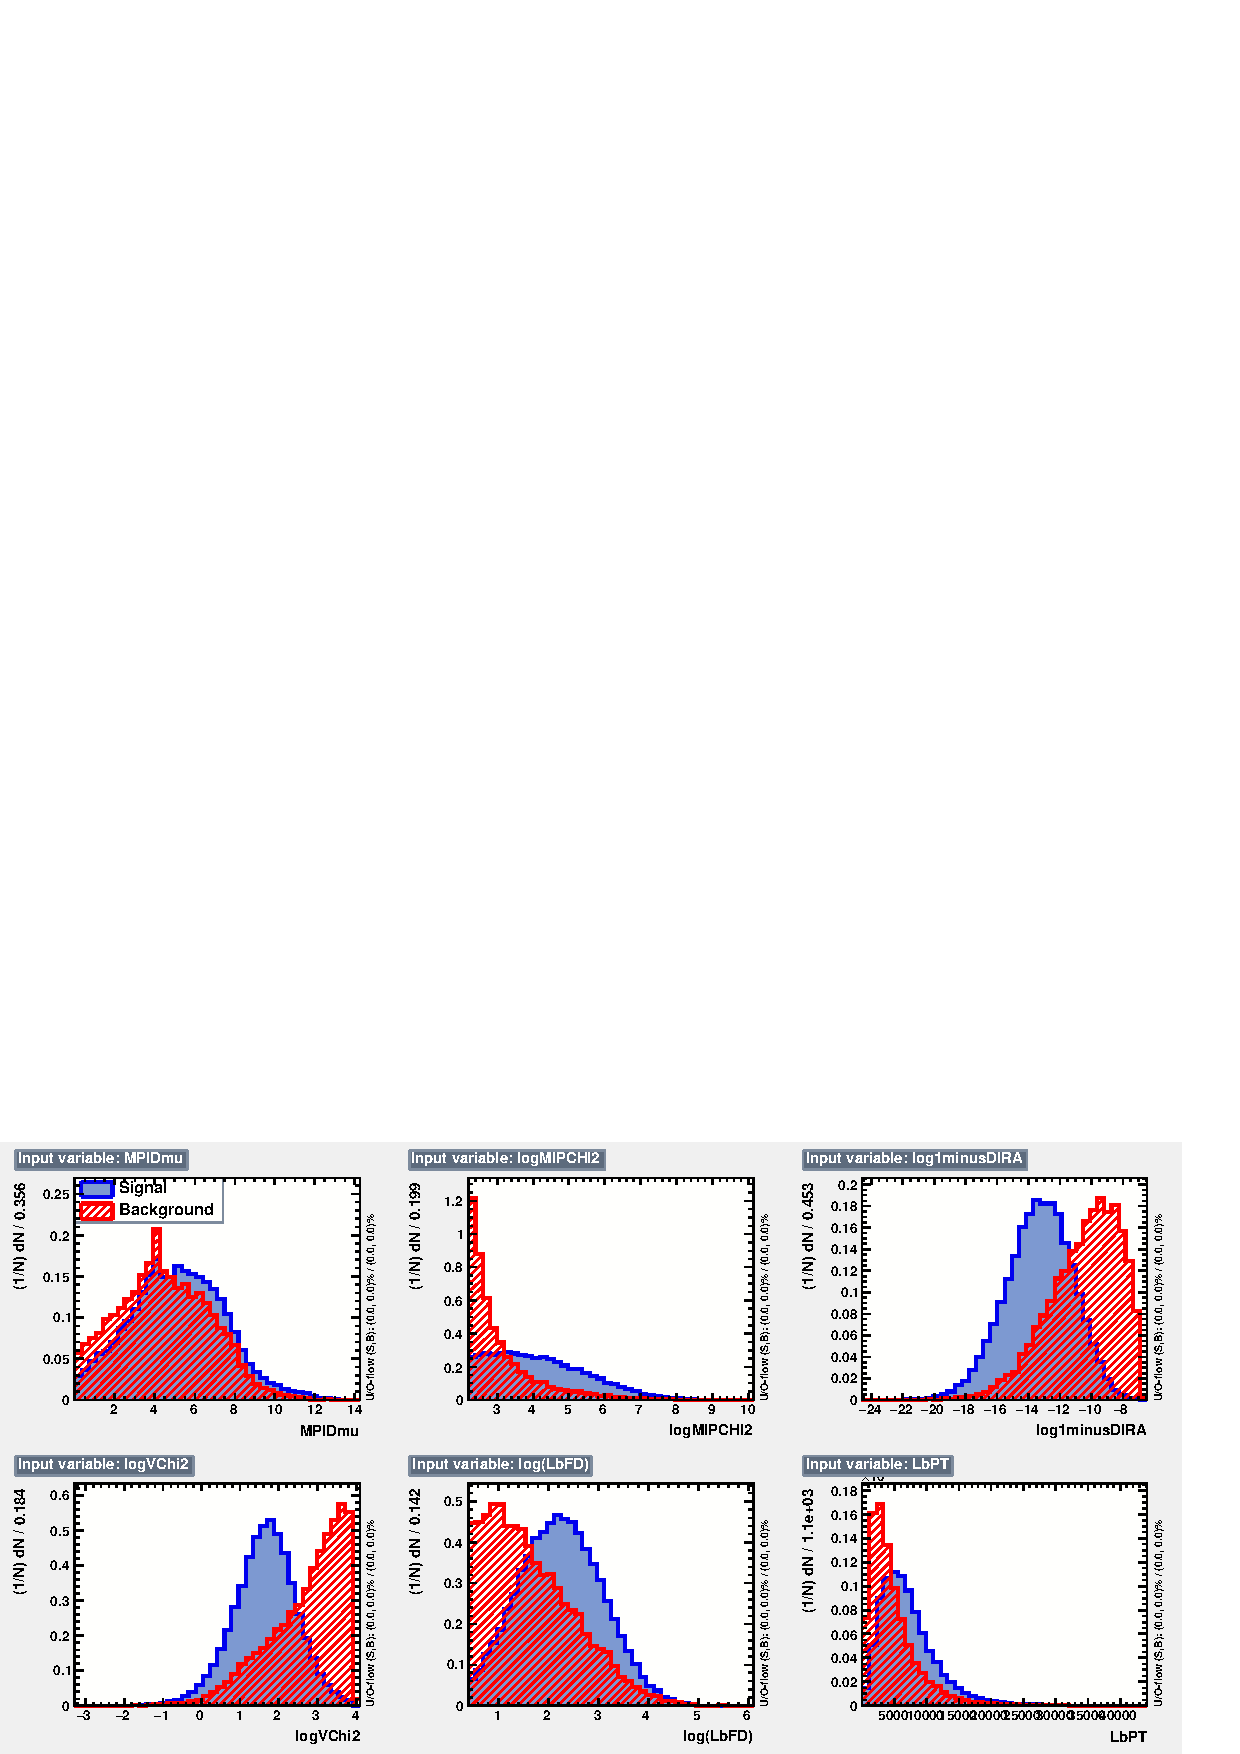
\includegraphics[scale=0.8]{Figures/05_open_charm/02_selection/variables_id_c1.pdf}\\% 
\vskip -0.04cm
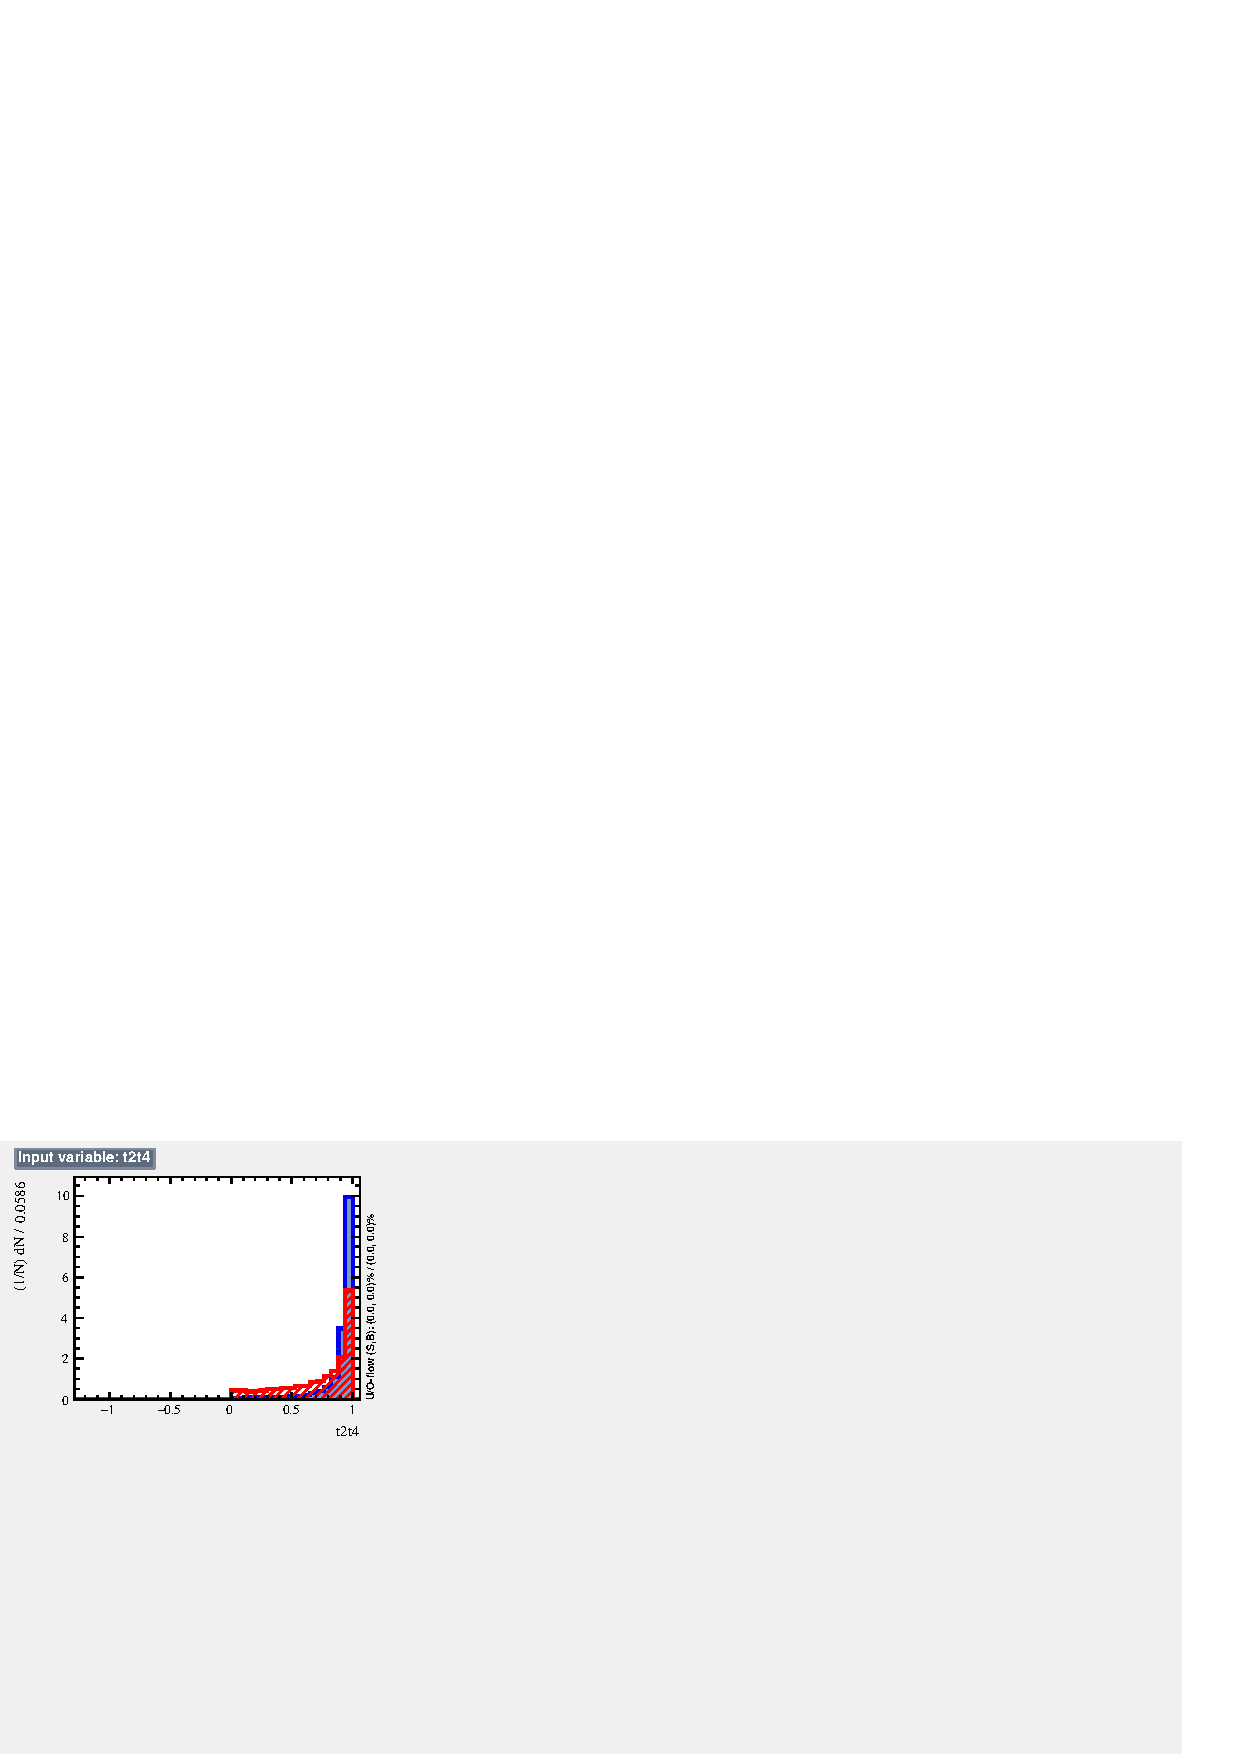
\includegraphics[scale=0.35]{Figures/05_open_charm/02_selection/variables_id_c2.png}%
\vskip -0.0cm
\caption{Distributions of variables used in BDTG for \LbLckkpi decays.}
\label{fig:BDTGvariables}
\end{figure}

\begin{figure}[!bth]
\centering
   \includegraphics[width=0.45\textwidth]{Figures/05_open_charm/02_selection/CorrelationMatrixB.pdf}%
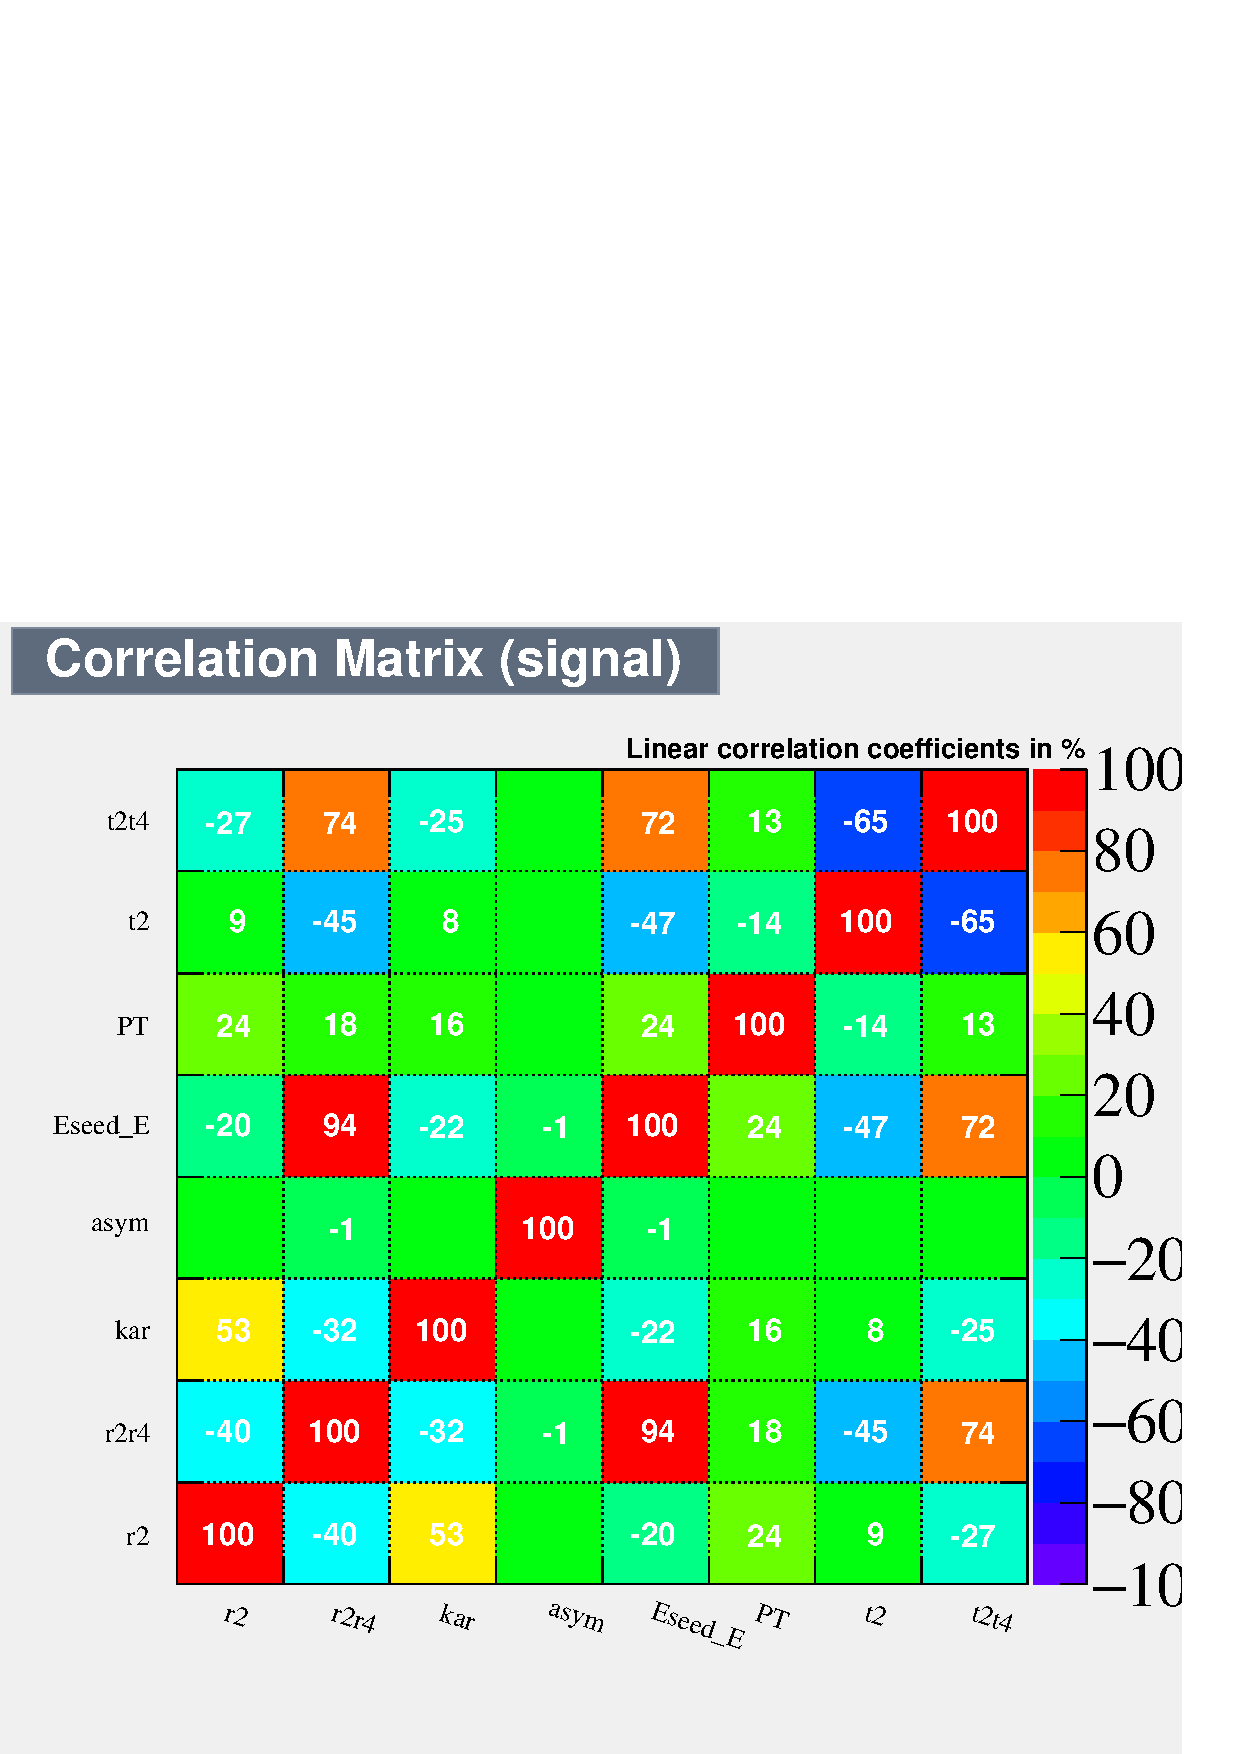
\includegraphics[width=0.45\textwidth]{Figures/05_open_charm/02_selection/CorrelationMatrixS.pdf}\\%
\caption{Correlation matrix of the training variables with TMVA toolkit for \LbLckkpi decays for the background (left) and the signal (right).}
\label{fig:corr}
\end{figure}


\begin{table}[!bth]
\centering
\caption{Rank of MLP trained variables}
\vspace{0.2cm}
\label{tab:rank}
\begin{tabular}{c c c}\hline\hline
Rank&variable&Importance\\\hline
1& Min \pt of K from \Lb & 0.0980 \\
2& Sum \pt of \Lb batch particles & 0.0955 \\
3& \pt of batch \pim & 0.0881 \\
4& Min $\log$($\chi^2_{IP}$ of K) & 0.0856 \\ 
5& $\log$(\Lb $\chi^2_{vtx}$) & 0.0794 \\
6& $\log$(\Lb $\chi^2_{IP}$) & 0.0777 \\
7& Min $\log$(\Lc daughter $\chi^2_{IP}$) & 0.0765 \\
8& Sum \pt of \Lc daughter & 0.0762  \\
9& $\log$(\Lb $\chi^2_{FD}$) & 0.0748 \\
10& $\log$($\chi^2_{IP}$ of \pim from \Lb) & 0.0777 \\
11& $\log$(\Lc $\chi^2_{vtx}$) & 0.0709 \\
12& $\log$(\Lb DIRA) & 0.0573 \\
13& z(\Lc)-z(\Lb) & 0.0472 \\
\hline \hline
\end{tabular}
\end{table}

The distributions of the BDTG and MLP classifier for signal and background are shown in Figure.~\ref{fig:overtrain_BDTG}. 
Both MVA classifiers don't have obvious overtraining and using MLP technique can get more consistent distributions between the training and test samples.  

\begin{figure}[!bth]
\centering
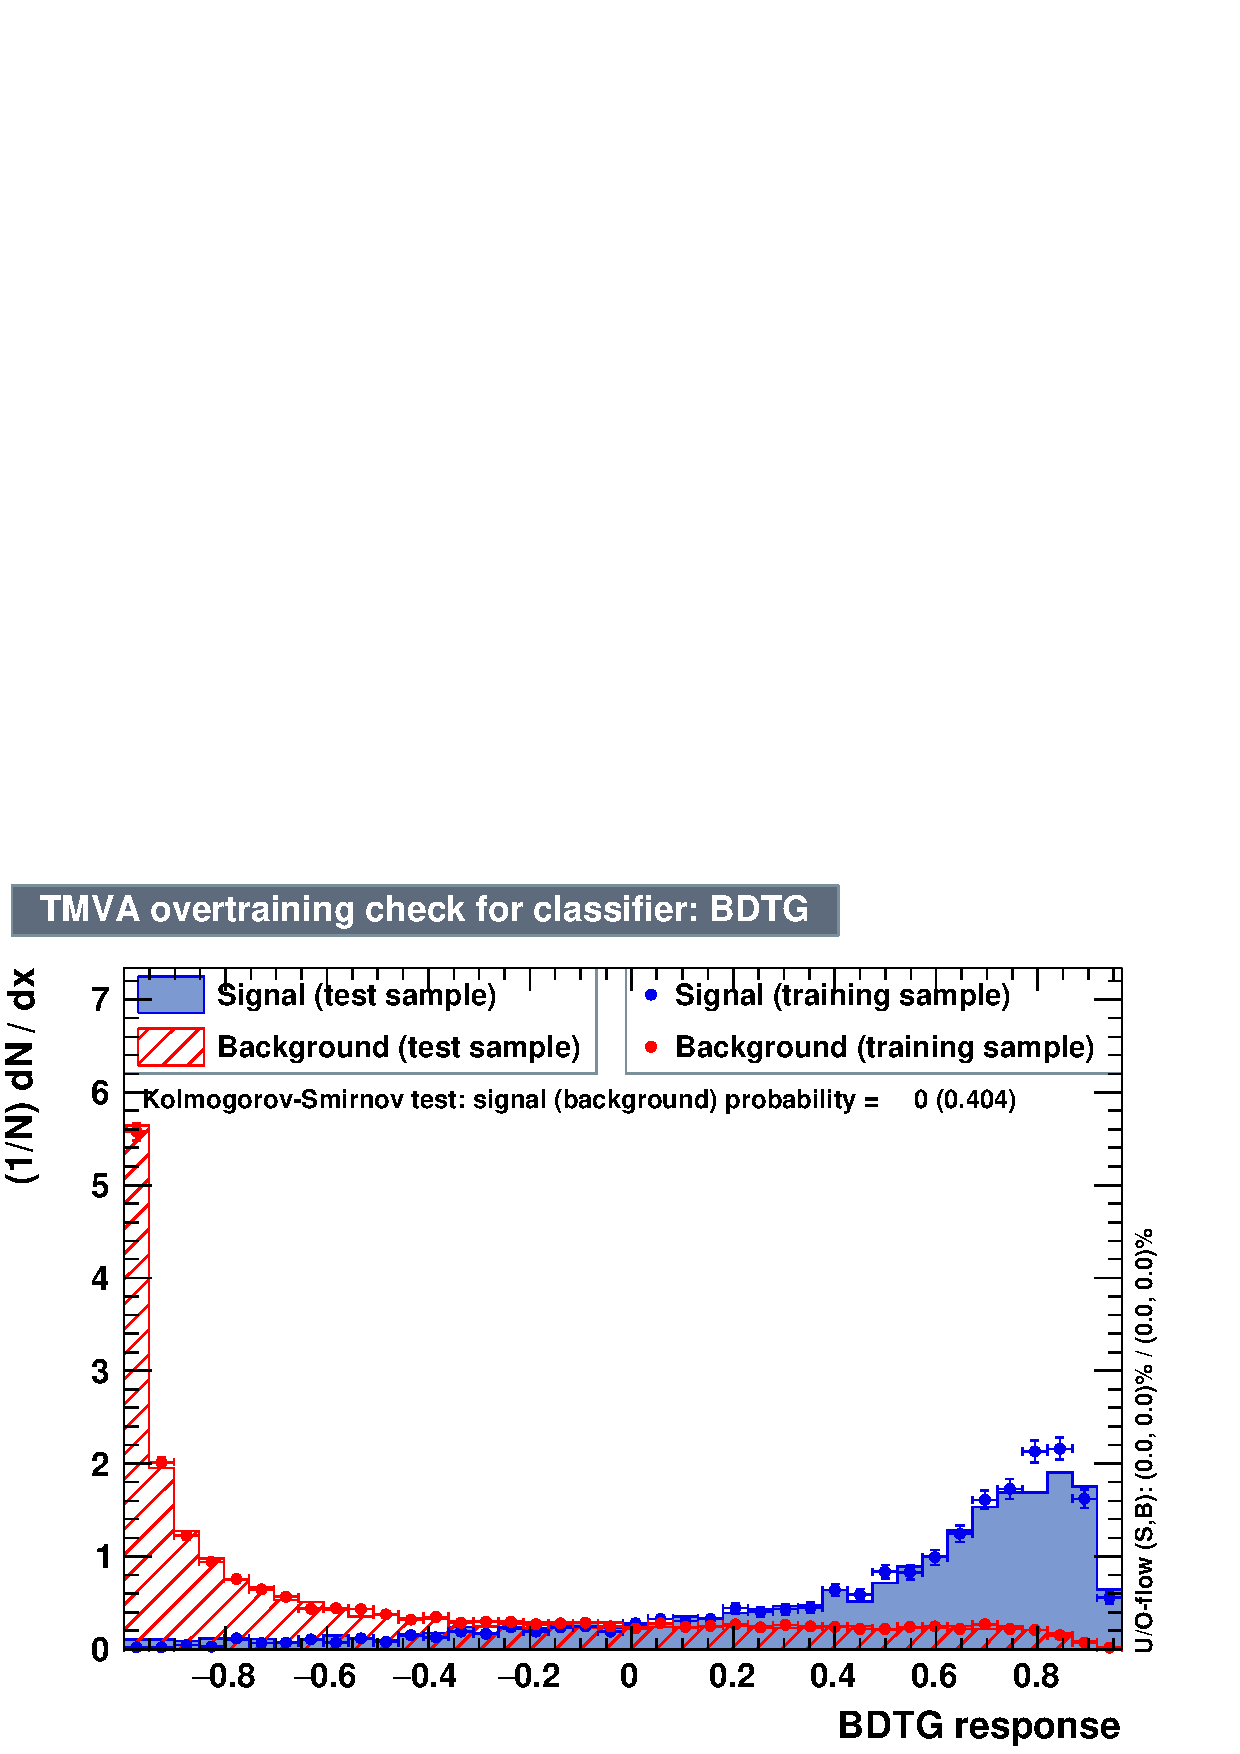
\includegraphics[width=0.45\textwidth]{Figures/05_open_charm/02_selection/overtrain_BDTG.pdf}%
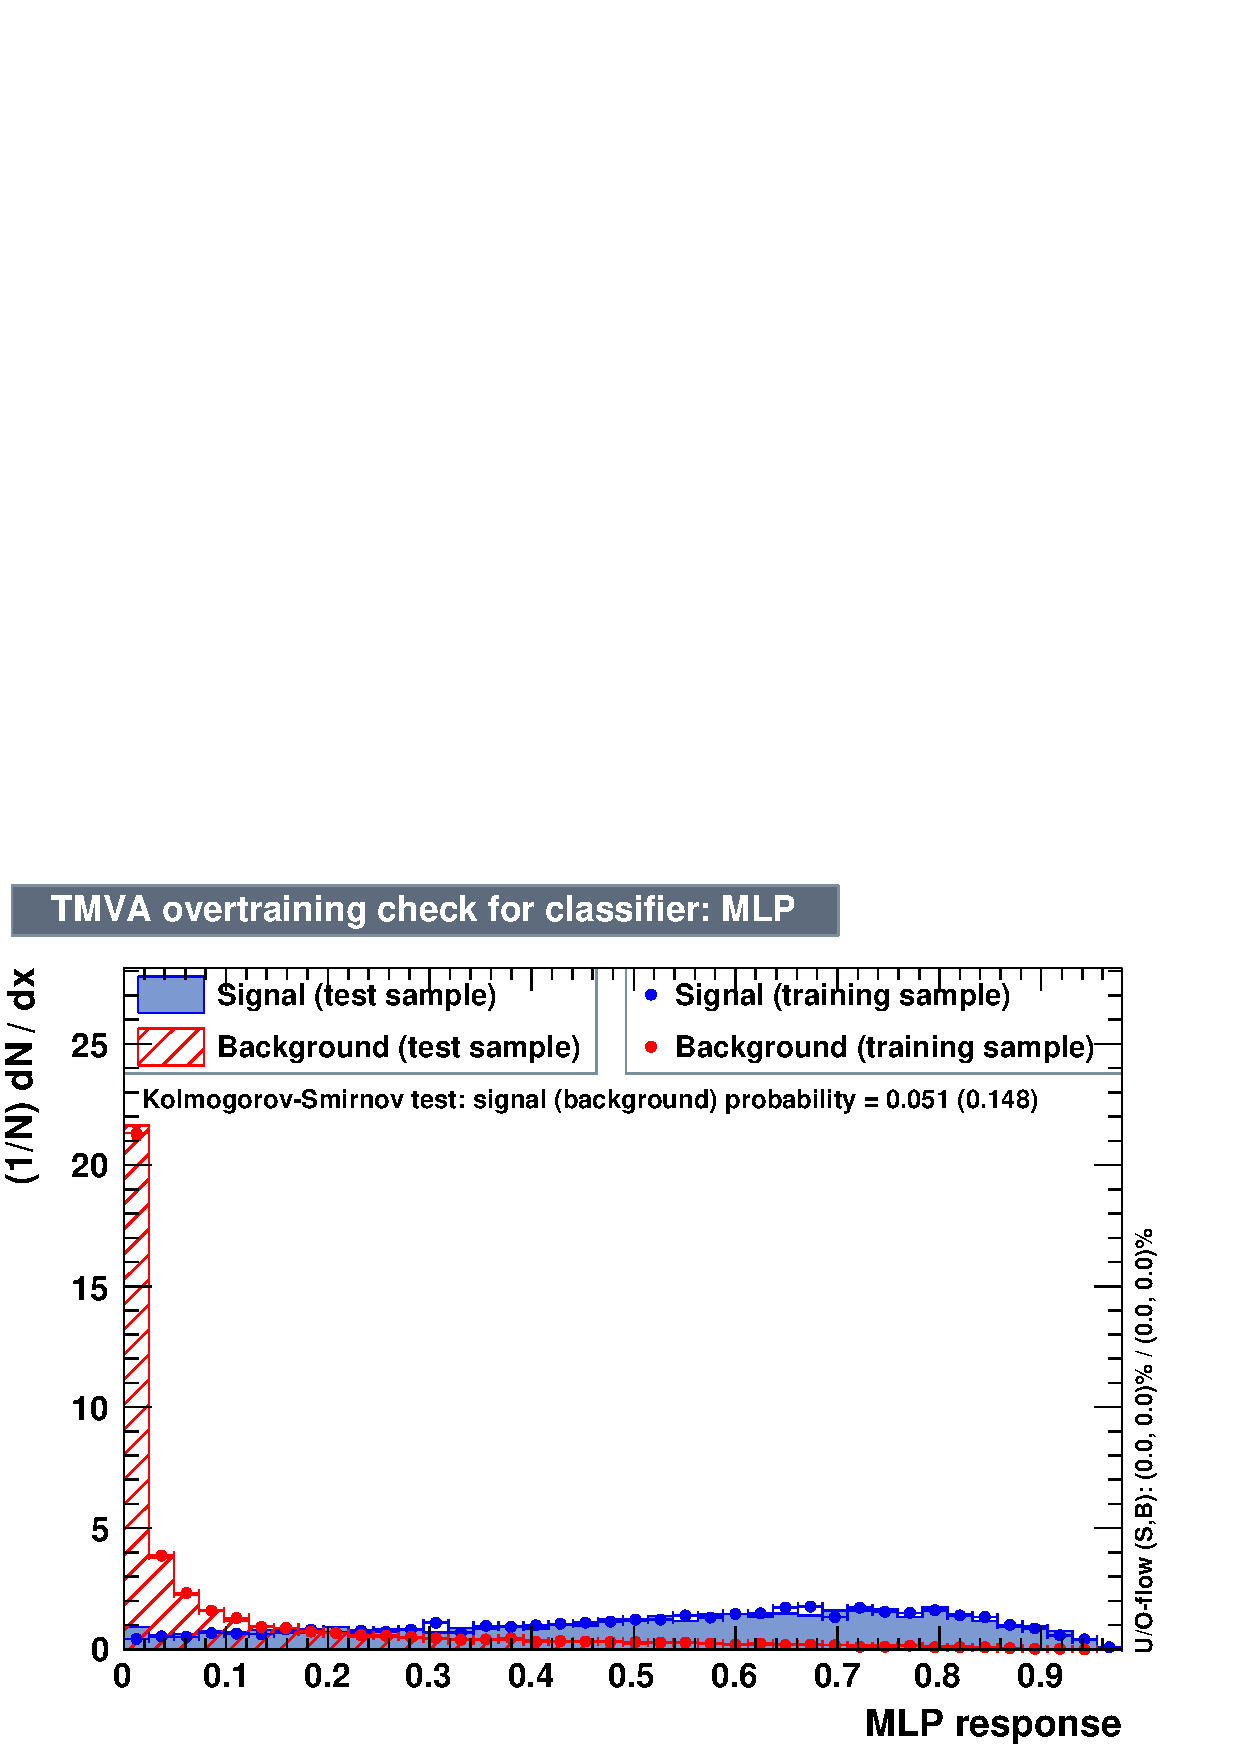
\includegraphics[width=0.45\textwidth]{Figures/05_open_charm/02_selection/overtrain_MLP.pdf}%
\caption{BDTG (left) and MLP (right) distributions for the signal and background for \LbLckkpi decays.}
\label{fig:overtrain_BDTG}
\end{figure}

\begin{figure}[!bth]
\centering
\includegraphics[width=0.45\textwidth]{Figures/05_open_charm/02_selection/mvaeffs_BDTG.pdf}%
\includegraphics[width=0.45\textwidth]{Figures/05_open_charm/02_selection/mvaeffs_MLP.pdf}%
\caption{Curves showing the signal and background efficiencies as a function of the BDTG (left) and MLP (right) cut value for signal channel.}
\label{fig:BDTG_optimize}
\end{figure}

An optimal cut point on the BDTG and MLP response is determined by maximizing the signal significance, $S/\sqrt{S+B}$, 
where $S$ ($B$) is the expected signal (background) yield in signal region, 
which is $\pm3\sigma$ ($\pm30$\mev) of the known $\Lb$ mass~\cite{PDG}. 
The initial yield for signal and background, $S_0$ and $B_0$, 
are estimated by using the mass spectrum of \Lb without BDTG or MLP requirements. 
The initial signal yield is estimated by fitting the $\Lb$ mass in signal region($5490$ \mevcc $<m(\Lb)<$ $5750$) 
with a DSCB(double-sided crystal ball) function for signal and a exponential function for background. 
With the these initial yields and the efficiencies of BDTG or MLP response of signal (MC) and background (sideband) samples in Figure.~\ref{fig:overtrain_BDTG},
we can derive the relation between BDTG or MLP cut threshold and the signal significance, 
which is shown in Figure.~\ref{fig:BDTG_optimize}. 
Using MLP technique, we can get larger significance.

\begin{figure}[!bth]
\centering
\includegraphics[width=0.45\textwidth]{Figures/05_open_charm/02_selection/rejBvsS.pdf}%
\caption{ROC curves for different MVA methods for signal channel.}
\label{fig:ROC}
\end{figure}

To maximize the signal significance, 
the BDTG and MLP working points are evaluated independently. 
The ROC curves of the results of different training methods are given in the Figure.~\ref{fig:ROC}. 
We find the MLP method is more powerful to discriminate the background and signal, 
with a larger significance and less overtraining effect and hence we use the MLP as the default method. 
And a value of 0.35 is determined as the default working point with a significance about 69.10 using MLP method. 

For the normalization channel \LbLcDs, 
the BDTG and MLP weights obtained in the signal mode are used to evaluate the MVA outputs. 
To take into account the difference of nodf between the signal mode and \LbLcDs, 
this variable is adjusted to distribute as $\chi^2$ with nodf=5. 
%The distributions are shown in Figure.~\ref{fig:compare_kkpi_ds}. 
Signal and background with the process like \LbLckkpi is estimated and determined as 0.09 for MLP cut. 
%corresponding plots are shown in Figure.~\ref{fig:BDTG_optimize_normalize}. 

\subsection{Potential Resonances}

Resonant contributions are expected in the signal decay \LbLckkpi, 
which are studied by the two body invariant mass distributions. 
In Figure.~\ref{fig:KpPi}, 
the 2-dimensional distributions are shown, 
and \Kp\pim decays are identified in the $K^{*}\to$\Kp\pim mass spectrum, 
and the \Lb mass window in $\pm30$\mev is applied.

\begin{figure}[!bth]
\centering
\includegraphics[width=0.45\textwidth]{Figures/05_open_charm/02_selection/kkpi_kpi.pdf} \\
\includegraphics[width=0.45\textwidth]{Figures/05_open_charm/02_selection/lckp_kpi.pdf}%
\includegraphics[width=0.45\textwidth]{Figures/05_open_charm/02_selection/lckm_kpi.pdf}%
\caption{2-D distribution of combined invariant mass.}
\label{fig:KpPi}
\end{figure}





